\bookchapter{第三十七章：範式之革——自「作碼」至「指 AI 作碼」}

\chapterintro{賀爾，展此書者，正立於職業範式之革之中央。為革之起，乃 2025 年一程序員於社交之媒所發之一言。聞之似近戲劇乎？然事實固如為也。}

\booksection{一、Vibe Coding 之誕生：一言所起之運動}

2025 年二月，Andrej Karpathy——其名請先識之，後尚數見之——於社交之媒發一推文，後為人所屢引：「有一新編程之法，曰 Vibe Coding，爾全憑感（vibes）而行，略碼之細節，使 AI 包攬一切。爾見何言何，複製而粘之，大抵能用即止。」

此言似脫口而出，實精名一已悄然生之範式之移：人不復逐行作碼，而以自然之語述其意，使 AI 成其實。Karpathy 之措辭微含戲謔，然其後有深察焉：AI 生碼之力既逾一閾，編程之隘，不復於「此行吾能作否」，而於「此事吾思之審否」。

\begin{tcbinfo}{小識：Vibe 何謂也？}
Vibe 直譯為「氛、感」。Vibe Coding 者，「隨感而指 AI 編程」也——爾述所欲，AI 任其實。識此詞，為革之「出生之證」也。

\end{tcbinfo}

自彼時始，「編碼」之義始分：舊之編碼，譯設計為語法；新之編碼，譯意為令。前者試指，後者試腦。

Vibe Coding 之詞，驟自戲謔而為嚴肅工程之念。至 2026 年之中，已自社交之媒一梗，演為一套完備之方法論——自需求之表、上下文之管、迭代之驗至質量之保，全流程悉涵焉。人亦悟：「憑感」者，入門之態也；真高效之 AI 編程，須系統之思維。而此思維之系，即此書所欲授爾者也。

\booksection{二、2026 年之勢：Agentic Engineering 之世}

至 2026 年八月，AI 編程之域已歷數要範式之迭代。Vibe Coding 者初火也，然眾旋覺：徒「憑感」而與 AI 語，所生之碼，質至不穩——時而驚豔，時而傾覆。於為範式始進：自簡之對話式編程，趨結構化之 Agent 工程。

又 Karpathy 也，2026 年之初，倡 Agentic Engineering 之念。異乎 Vibe Coding「言出即生」者，Agentic Engineering 所重者：予 AI 一之，使自規其步、調其器、驗其果、迭而正之。AI 不復徒生碼之器，乃能感境、能決策、能行事之智能體（Agent）也。

此變有三要焉：

\begin{enumerate}
  \item 交感之式變：自「一問一答」變為「既設其之而授權」。
  \item 工之所產變：自「一段之碼」變為「一完整之項目」。
  \item 人之所任變：自「逐行審碼」變為「定其界、驗其果」。
\end{enumerate}

數不誣也：Cursor 於 2026 年四月所頒之 Cursor 3 中，Agent 模式之使用率首超 Tab 補全之式，為開發者已大規模趨此工法之徵；而 Claude Code 者，終端原生 AI 編程之器也，至 2026 年之中，年化之入已達二十五億美元之規模。下之趨勢圖，可使爾親睹此交會之時：

\begin{center}
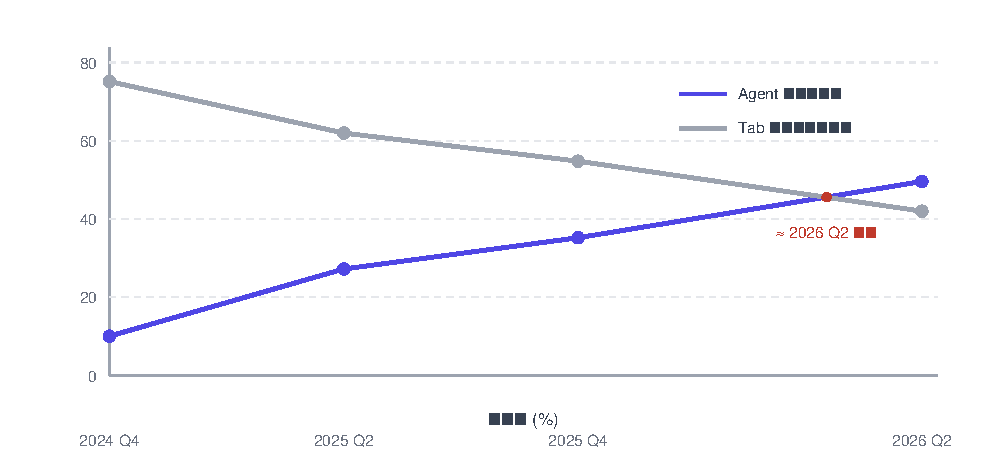
\includegraphics[width=0.92\linewidth]{figures/fig-di-san-shi-qi-zhang-1}
\\[2pt]\small 圖一：AI 編程交感模式使用率之趨勢（據行業調研之數估算，2026 Q2 Agent 模式超 Tab 補全）
\end{center}

然實言之：器與模型之變，表象也。無論爾用 Cursor 抑 Claude Code，無論底層之模型為 GPT-5 抑 Claude 4.5，成之者皆循同一底層之方法論。此本指南所欲授爾者也。

\booksection{三、核心之悟之變：自 Coder 至 Conductor}

舊之編程之教，授爾為 Coder——解語法、記 API、調邏輯之誤。AI 編程之世，此任方被重定。爾不復須親作每行之碼，然須為「指揮官」（Conductor）：定戰場、立規則、分其任、驗其成。

此變之核，不於「爾能作碼否」，而於「爾能思審所欲為否」。良將不必為至勇之卒，然必最審戰之之、地之形、兵之布。同理，善 AI 編程者不必通每種編程語言之細，然必最審項目之之、架構之限與質量之準。

此表宜爾再觀——為變之全義，盡括於斯：

\begin{center}
\begin{tabularx}{\linewidth}{|X|X|X|}
\hline
\textbf{維度} & \textbf{舊之 Coder} & \textbf{AI 之指揮官（Conductor）} \tabularnewline
\hline
核心之技 & 記語法、調 API、除誤 & 定需求、管上下文、斷驗收 \tabularnewline
工之方式 & 逐行作碼 & 述其意，審其產 \tabularnewline
質量之控 & 己所作者，己心有數 & 以測試與審查驗 AI 之產 \tabularnewline
所需之知 & 深通特定之語言、框架 & 廣識技術之全貌，深解業務之邏輯 \tabularnewline
隘之所於 & 編碼之速與語法之記 & 思之審與達意之能 \tabularnewline
誤之所自 & 語法之誤、邏輯之漏 & 需求之晦、上下文之乏 \tabularnewline
\hline
\end{tabularx}
\end{center}

\begin{center}\small\color{gray}舊 Coder 與 AI 指揮官之能維之比\end{center}

此非謂編程之知不足重也。正相反：能解 AI 所作之碼，方能審而正之；解數據之構與算法，方能斷 AI 之策合理否。知之所積，定爾「指揮之上限」——然知之所任，自「執行之器」變為「決斷之據」矣。

\booksection{四、方法論何以重於工具}

器三月一迭代，方法論三年一進化。習一器之操作，三月後或已陳；得一思維之法，三年後猶可用。

多人初學 AI 編程，首問「何器至善」「何模型至強」。此問非不重要，然所問之序誤矣。2026 年八月之器局，與 2025 年八月迥異——Trae、Qoder 諸器興衰起伏，Cursor 自插件而為獨立之 IDE，復進至 Cursor 3；Claude Code 自實驗之案而為終端編程之主流。然劇變之後，成者所循思維之則，幾無所變。

為故此書不惜費篇幅於某器之細操——此等之內容，甫成即陳舊。反之，全書之重，盡於一套已驗之思維方法論：何以思需求、何以與 AI 通、何以驗其產、何以續而迭代。得此法，則易任何之器皆可速上手；徒學器之操，一易其器，則自零始矣。

\begin{tcbinfo}{慰零基之讀者}
爾若零基，毋為「方法論」三字所懾。方法論者，非玄之哲也，乃「遇事當何以思」之操作之冊也。譬之學庖：可循譜而步（器之操），然大庖所解者，「何以如此調味」「火候何以制」（方法論）也。此書自至基之念始，每一則皆配對比之案例，使爾非惟解「何謂」，更能得「何以為」。

\end{tcbinfo}

\begin{tcbpractice}{來動手：為今之爾攝一「角色之影」}
出紙一張，書三問之答：(1) 爾今何以用 AI 助爾作碼（若曾用之）？(2) 爾肖上表之「Coder」抑「指揮官」？(3) 爾望三月後之己，何以述其工法？書畢夾之書中，讀竟第四十七章復觀之——爾將見其變之速，逾於所想。

\end{tcbpractice}

\begin{tcbsummary}{本章小結}
\begin{itemize}
  \item 2025 年 Karpathy 以「Vibe Coding」名 AI 編程之革：自逐行作碼，變為以自然之語述意
  \item 2026 年進為 Agentic Engineering：與之之、授之權，AI 自規劃而行，人任驗收
  \item Cursor 3 之 Agent 模式使用率首超 Tab 補全；Claude Code 年化之入達二十五億美元
  \item 爾之新任為 Conductor（指揮官）：定戰場、立規則、分其任、驗其成
  \item 工具每三月一迭代，方法論每三年一進化——學方法論，勿徒學操作
\end{itemize}

\end{tcbsummary}
